%% Reykjavik University Presentation Template by Joseph T. Foley < foley AT ru DOT is >
\documentclass[aspectratio=169]{rubeamer}
%% Add option "icelandic" to switch sections and labels
%% Add one of these options to change the aspect ratio:
%% 1610 149 54 43 32 which is 16:10 14:9 etc.

%% If you have customizations and packages you use a lot, put them in custom-beamer.sty
%% It will be automatically loaded if it exists
%% I have loaded this with packages and macros I find useful


%%----------- Citations ---------------------------
%% I highly advise using JabRef to manage your .bib files.
%% It can catch a lot of errors early and helps you fill things in.
%% In particular, you probably want to set it to fix line endings to NL only in the preferences.

%%%% Now pick a citation style
%%IEEE citations (just numbers)
%\usepackage[backend=biber, bibencoding=utf8, style=ieee]{biblatex}

%% APA style (author, year) -- need all of these lines
%\usepackage[backend=biber, bibencoding=utf8, style=apa]{biblatex}
%\usepackage[american]{babel}
%\DeclareLanguageMapping{american}{american-apa}  % after biblatex and babel

%% Alphabetic (abbrv-year), more compact
\usepackage[backend=biber, bibencoding=utf8, style=alphabetic]{biblatex}

%% Put your reference library files here. Don't forget to put the .bib
%% extension. If you have multiple people with their own libraries (or
%% are using the Zotero plugin) it is a good idea to have multiple
%% files separated according to some agreement.  This is the divisions the author uses:

\addbibresource{references.bib}%references specific to this paper
\addbibresource{references-ad.bib}%reference related to Axiomatic Design
\addbibresource{references-foley.bib}%references that the author has participated on.  Helpful for writing a CV.
\addbibresource{references-collections.bib}%Due to BibTeX/Biber processing, multi-author books and proceedings must go last if they are used as crossref.


%% ------------------ Graphics ----------------------------%%
\graphicspath{{graphics/}{Graphics/}}
%% This is a list of folders to search for graphics files to include in that order.
%% Each path should be in a {}.  
%% Make sure that the upper/lowercase of the letters matches the folder or
%% you may have weird problems with partners using other operating systems.

\usepackage{datetime}

\newdateformat{monthyeardate}{\monthname[\THEMONTH] \THEYEAR}

%% -----------------Titles and Footers ---------------------%%
%% The abbreviated information goes in the [], the full information in {}
\title[RU Presentation]{Real Time, Onboard-only Landing Site Evaluation for Autonomous Drones}
\subtitle[demo]{PhD Thesis Proposal}
\author[Springer]{Joshua Springer}
\institute[RU]{Reykjavík University}
\date[2022]{\monthyeardate\today}%Set this to when you will present

\logo{
\includegraphics[width=1.5cm]{ru-logo}}
\titlegraphic{
\includegraphics[width=2CM]{ru-logo}}

\AtBeginSection[]{
  \begin{frame}
  \vfill
  \centering
  \begin{beamercolorbox}[sep=8pt,center,shadow=true,rounded=true]{title}
    \usebeamerfont{title}\insertsectionhead\par%
  \end{beamercolorbox}
  \vfill
  \end{frame}
}

\begin{document}
%----------- titlepage ----------------------------------------------%
\begin{frame}[plain]%plain option gets rid of the footer and the per-page logo
  \titlepage
%  \begin{textblock}{10}(12,4)
%    
\includegraphics[width=0.3\textwidth]{ru-logo}
%  \end{textblock}

\end{frame}

\begin{frame}
  \frametitle{Presentation Structure}
  \begin{enumerate}
    \item Introduction
      \begin{itemize}
        \item Problem Description
        \item Motivation
        \item State of the Art
      \end{itemize}
    \item Current Progress
      \begin{itemize}
        \item Completed/ongoing projects
        \item Challenges
      \end{itemize}
    \item Research Plan
      \begin{itemize}
        \item Methods
        \item Risk Analysis
      \end{itemize}
  \end{enumerate}
\end{frame}

%----------- slides ----------------------------------------------%
\section{Introduction}

\begin{frame}
  \frametitle{Problem Description and Motivation}
  \begin{columns}
    \column{0.5\textwidth}
    \begin{itemize}
      \item Most of drone flight has been \textbf{automated}.
      \begin{itemize}
        \item Takeoff
        \item Waypoint-to-waypoint-flight
        \item Miscellaneous tasks: track/orbit an object, take a picture, etc.
      \end{itemize}
    \item Landing is still done \textbf{manually}.
    \end{itemize}
    \column{0.5\textwidth}
    \centering
    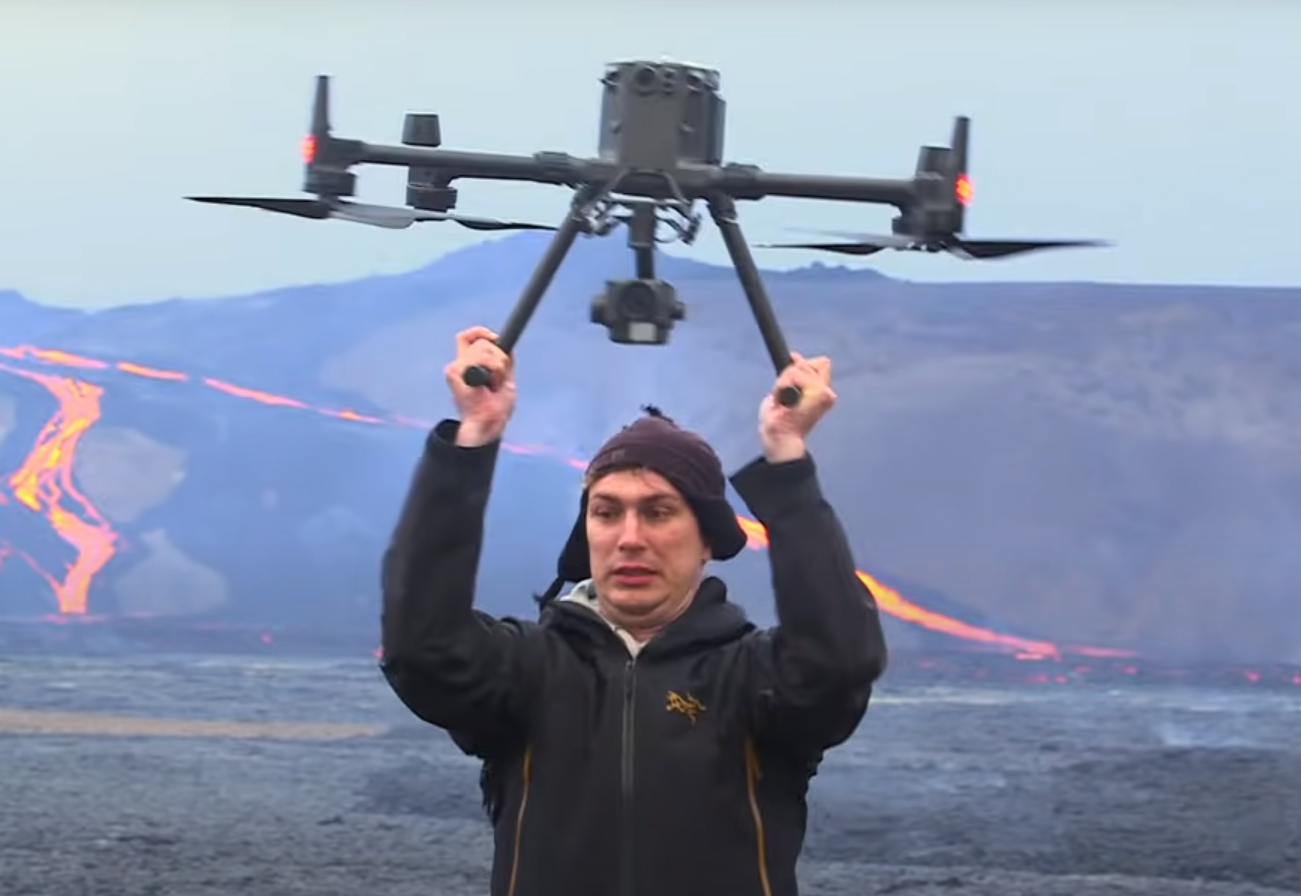
\includegraphics[width=0.75\textwidth]{human_assisted_landing}\\
    ``Human-assisted landing''
  \end{columns}
\end{frame}

\begin{frame}
  \frametitle{State of the Art}
\end{frame}

\section{Current Progress}

\begin{frame}
  \frametitle{Test Hexacopters}
  \begin{columns}
    \column{0.5\textwidth}
    \begin{itemize}
      \item Two Tarot 680 hexacopters
      \item For real-world proof of concept of master thesis simulations.
    \end{itemize}
    \column{0.5\textwidth}
    \centering
    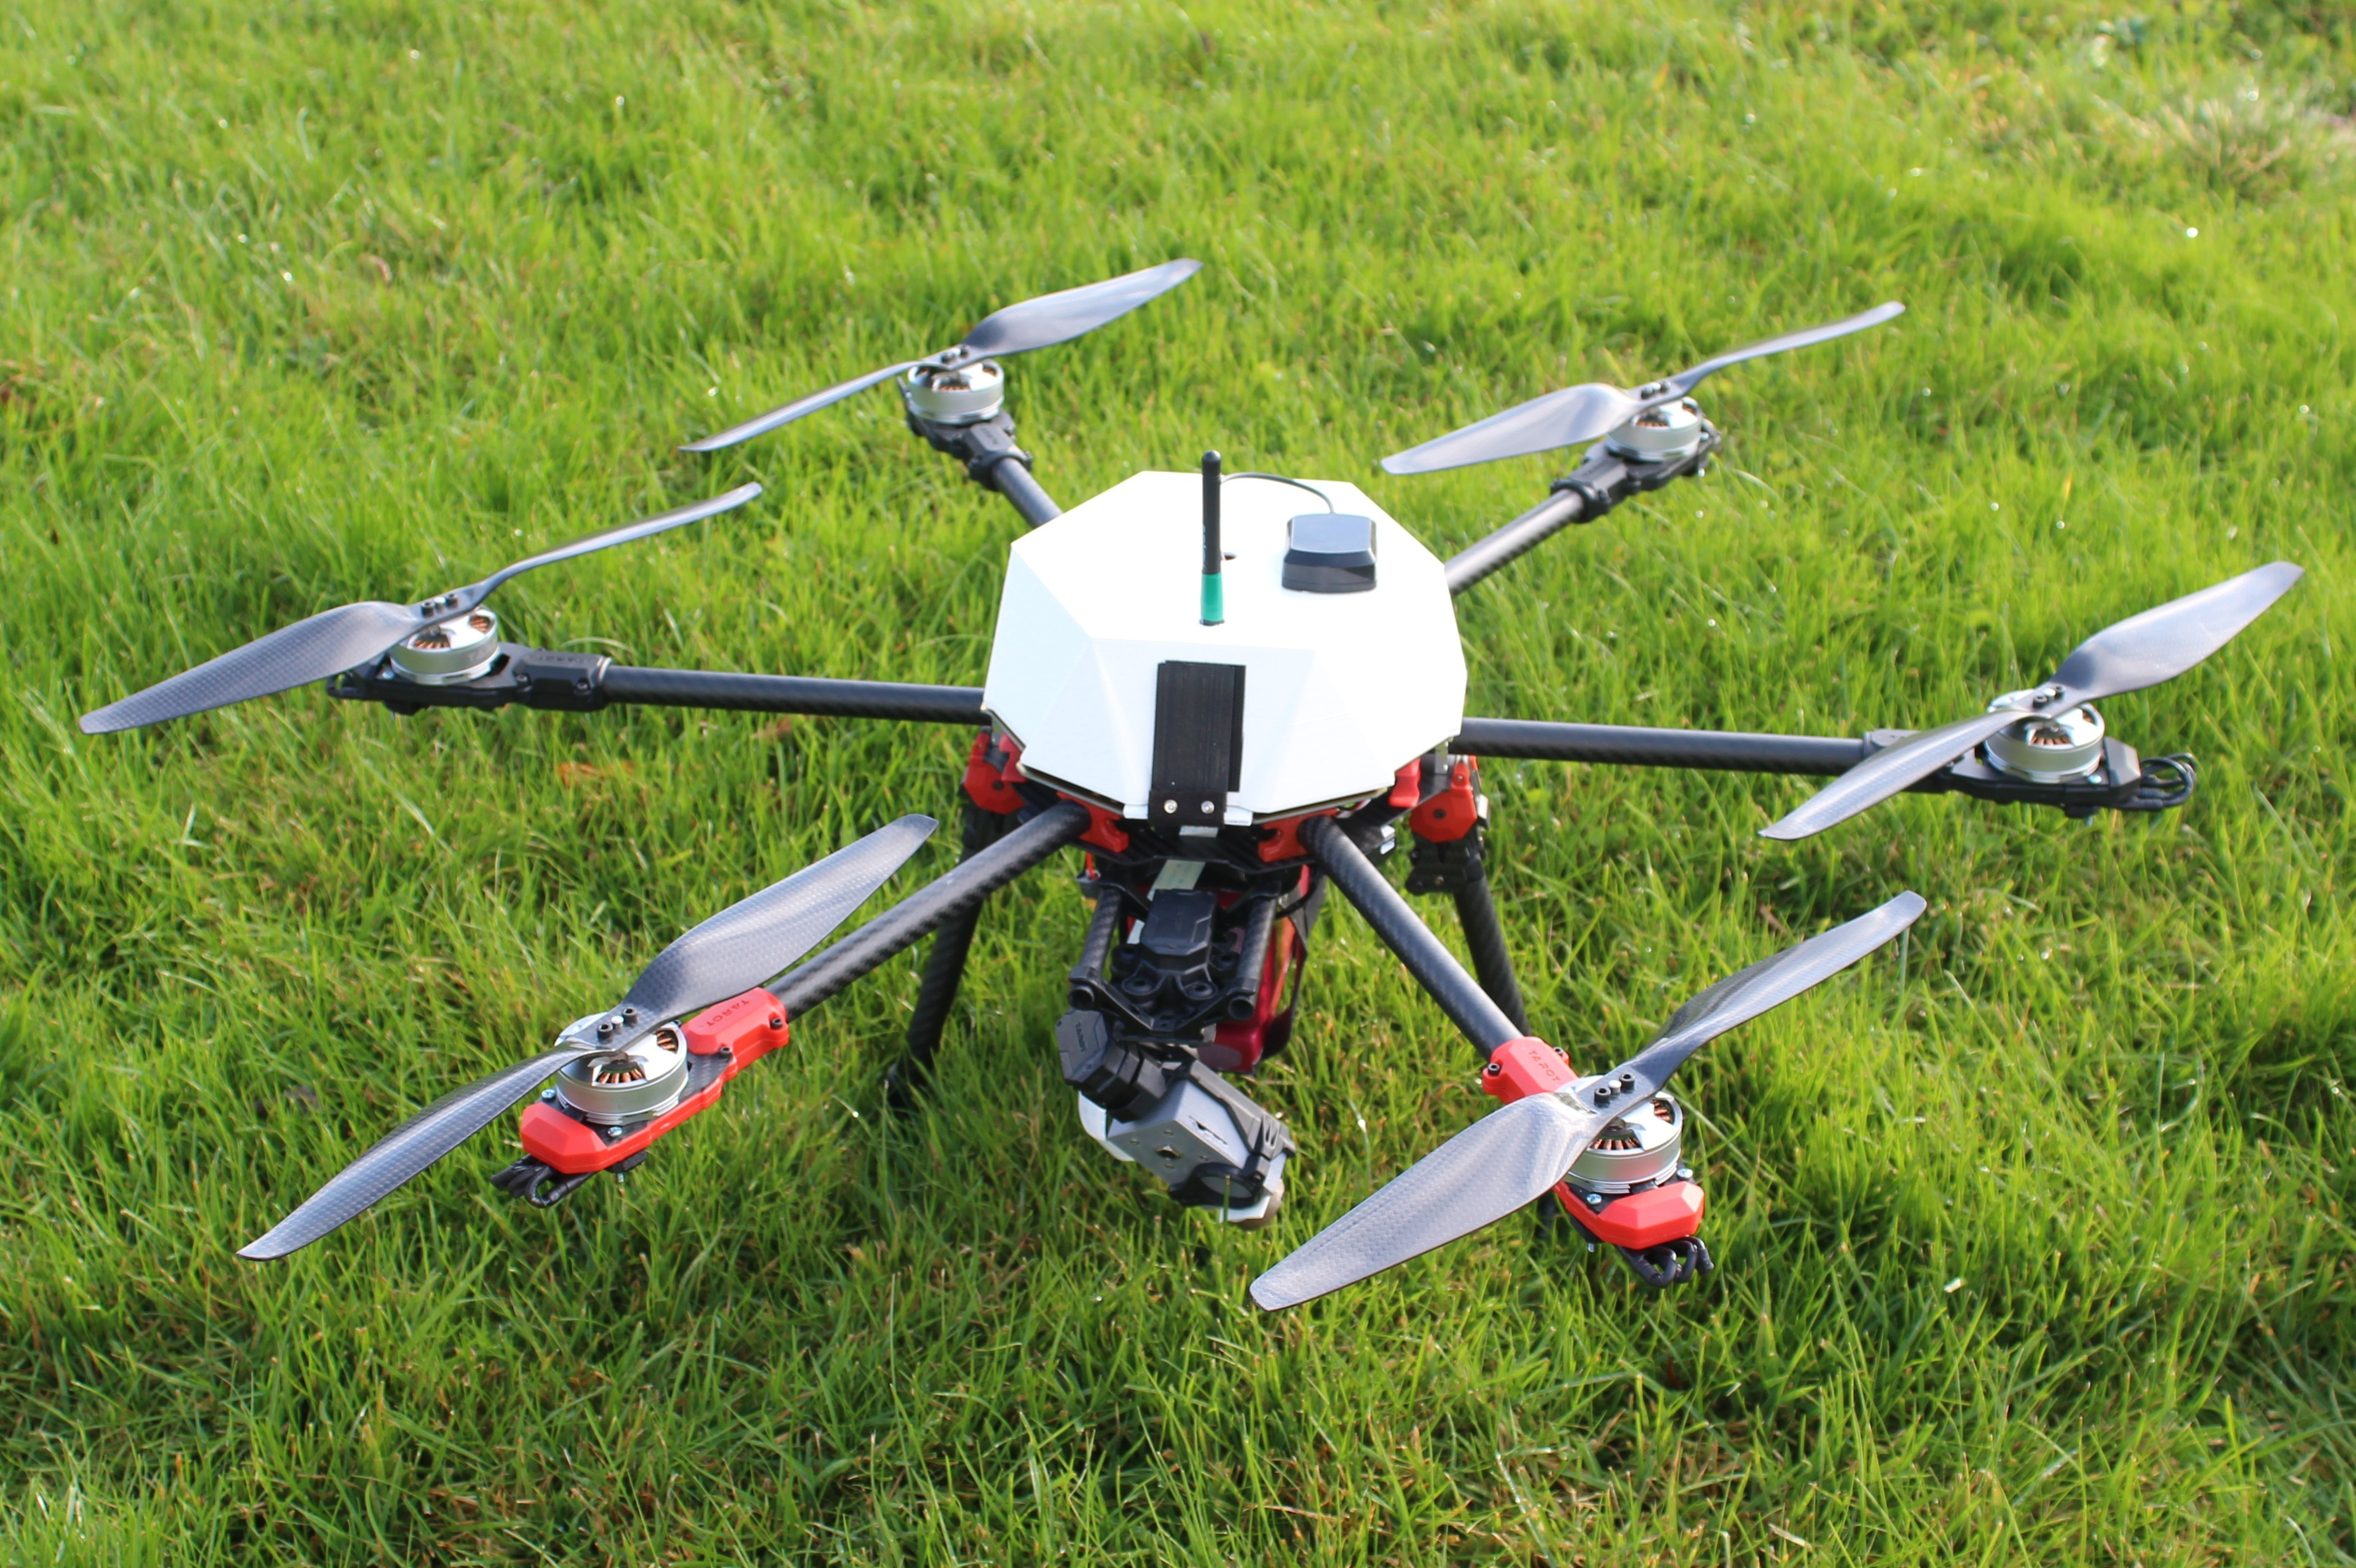
\includegraphics[width=0.75\textwidth]{coral_drone}\\
  \end{columns}
\end{frame}

\begin{frame}
  \frametitle{Test Hexacopters' Components}
  \begin{columns}
    \column{0.5\textwidth}
    \begin{itemize}
      \item Navio2 + RPi 3 autopilot combo
      \item Companion boards:
      \begin{itemize}
        \item Google Coral (embedded TPU)
        \item Jetson Nano (embedded GPU)
      \end{itemize}
      \item Gimbaled camera modules
      \item 433 MHz telemetry
      \item 2.4 GHz R/C control
    \end{itemize}
    \column{0.5\textwidth}
    \centering
    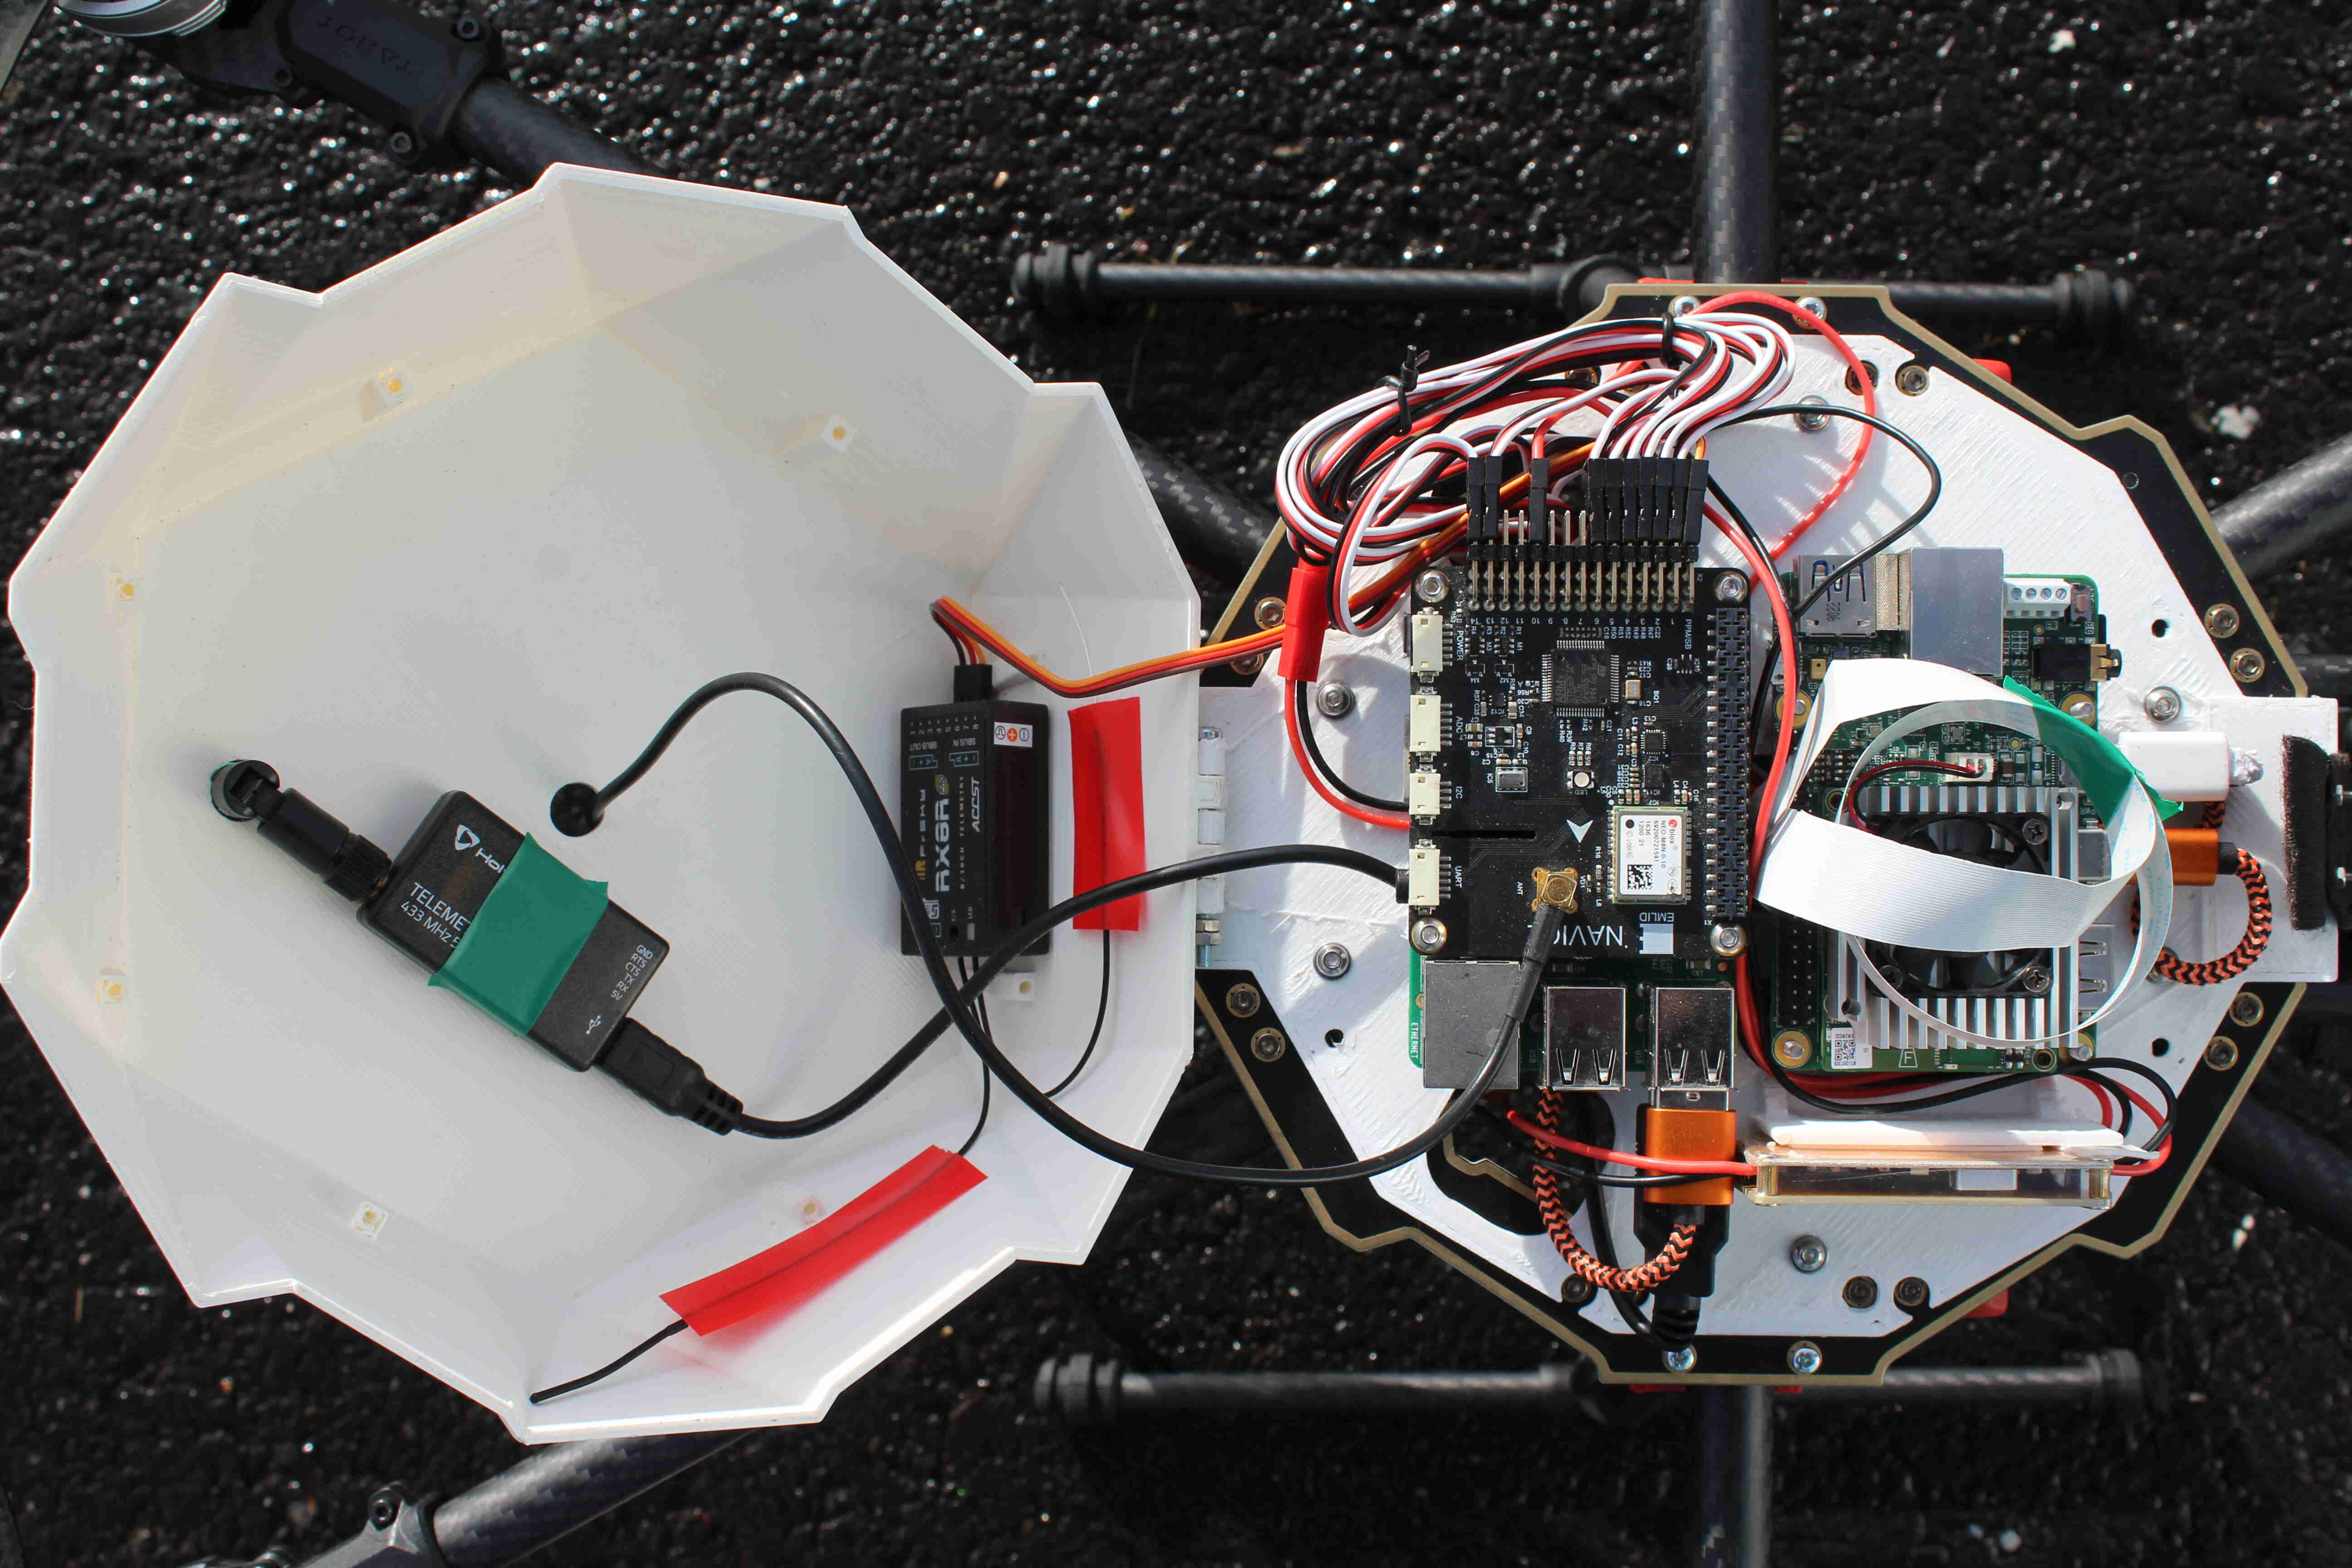
\includegraphics[width=0.6\textwidth]{coral_electronics}\\
    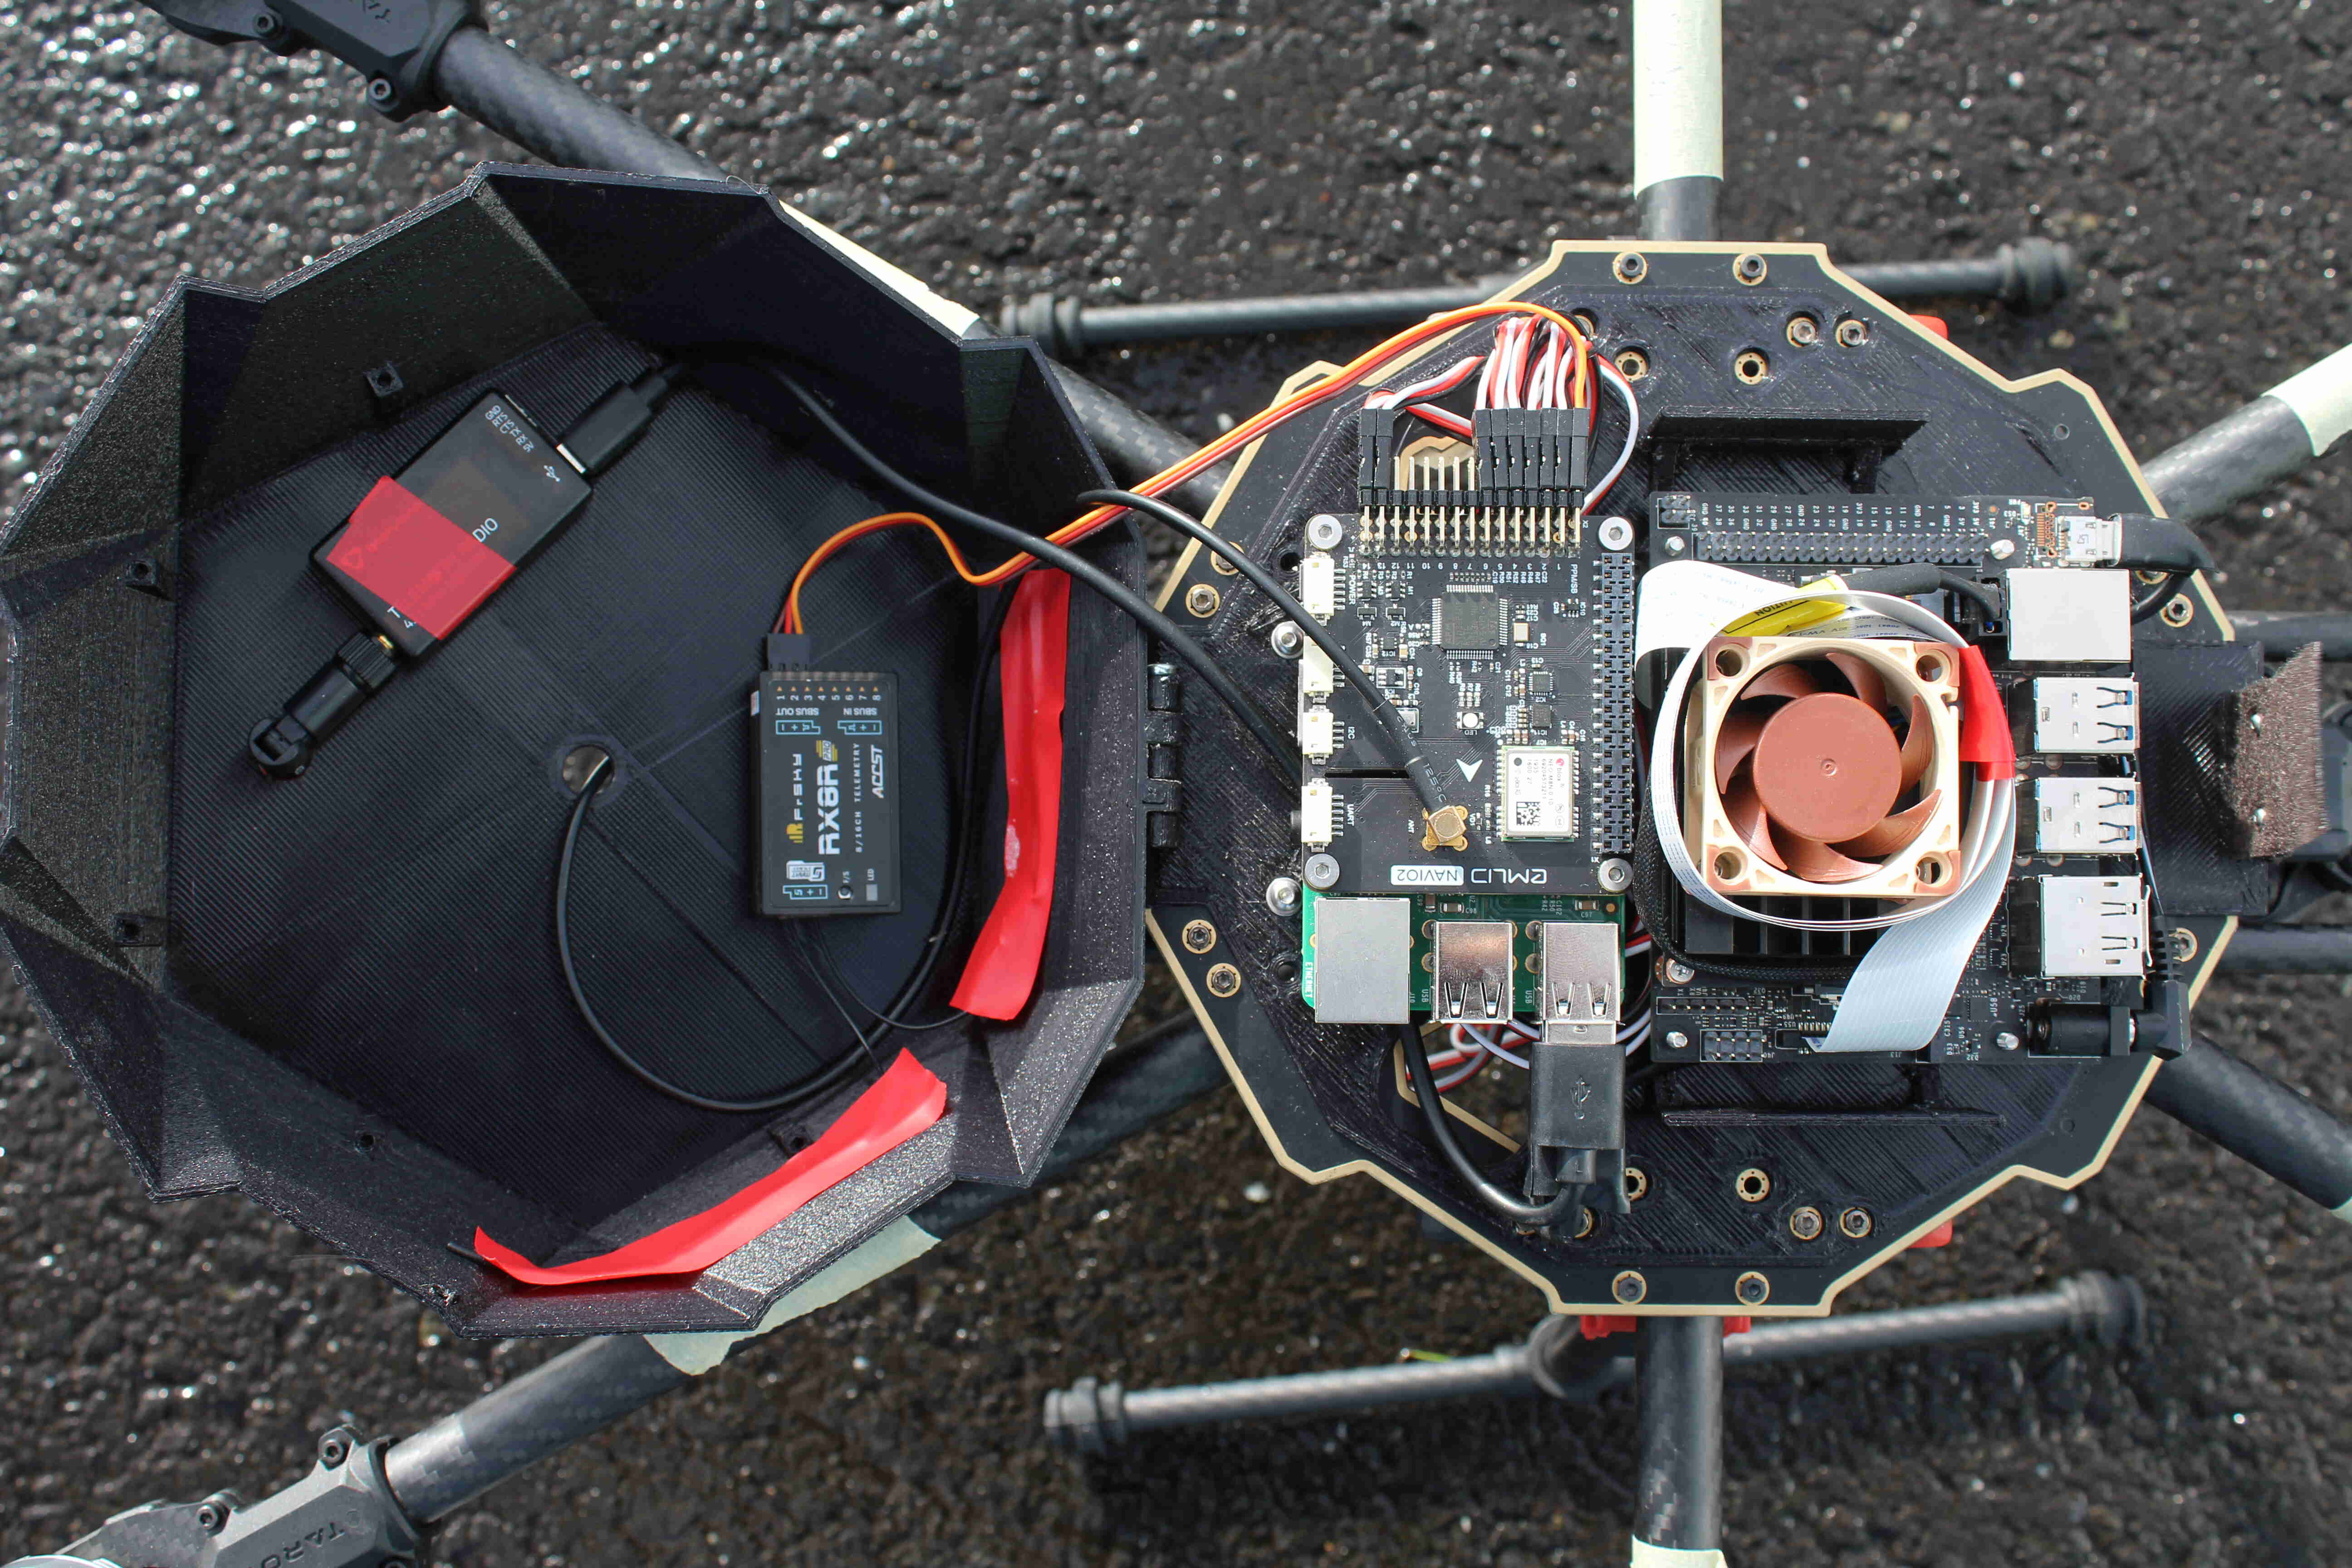
\includegraphics[width=0.6\textwidth]{jetson_electronics}\\
  \end{columns}
\end{frame}

\begin{frame}
  \frametitle{Test Hexacopters' Performance}
  \begin{columns}
    \column{0.5\textwidth}
    \begin{itemize}
      \item Stable flight performance
      \item > 20 min flying time
      \item Successful marker tracking
      \item Errors during approach
      \begin{itemize}
        \item Monocular pose estimation ambiguity
        \item GPS inaccuracy
      \end{itemize}
      \item No successful autonomous landing\\(but almost)
    \end{itemize}
    \column{0.5\textwidth}
    \centering
    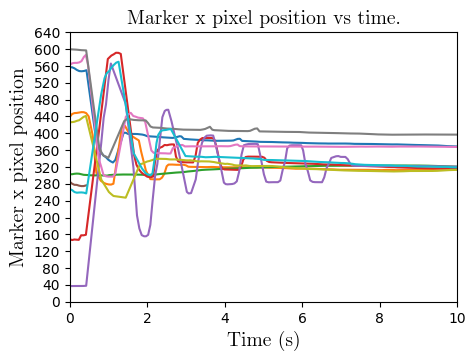
\includegraphics[width=0.6\textwidth]{coral_gimbal_performance_x_axis}\\
    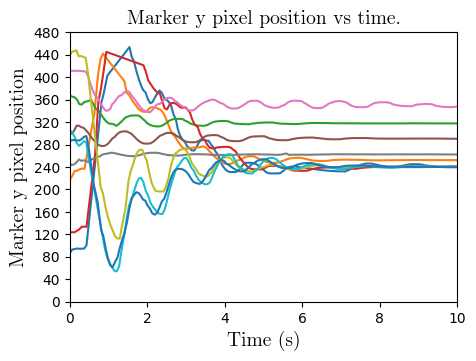
\includegraphics[width=0.6\textwidth]{coral_gimbal_performance_y_axis}\\
  \end{columns}
\end{frame}

\begin{frame}
  \frametitle{Fiducial System Modifications}
  \begin{columns}
    \column{0.5\textwidth}
    Necessary properties:
    \begin{itemize}
      \item Overcome orientation ambiguity
      \item Maintain visibility of the marker at both long- and short- distances
      \item Be adequately computationally efficient to run on embedded hardware.
    \end{itemize}
    \column{0.5\textwidth}
    \centering
  \end{columns}
\end{frame}

\begin{frame}
  \frametitle{Fiducial System Modifications: WhyCode}
  \begin{columns}
    \column{0.5\textwidth}
    \column{0.5\textwidth}
    \centering
  \end{columns}
\end{frame}

\begin{frame}
  \frametitle{Fiducial System Modifications: April Tag}
  \begin{columns}
    \column{0.5\textwidth}
    \column{0.5\textwidth}
    \centering
  \end{columns}
\end{frame}

\begin{frame}
  \frametitle{Fiducial System Modifications: Performance Analysis}
  \begin{columns}
    \column{0.5\textwidth}
    \column{0.5\textwidth}
    \centering
  \end{columns}
\end{frame}

\begin{frame}
  \frametitle{Heavy Lift IR Drone}
  \begin{columns}
    \column{0.5\textwidth}
    \column{0.5\textwidth}
    \centering
  \end{columns}
\end{frame}

\begin{frame}
  \frametitle{Autonomous Landing Proof of Concept \textbf{(FINALLY!)}}
  \begin{columns}
    \column{0.5\textwidth}
    \column{0.5\textwidth}
    \centering
  \end{columns}
\end{frame}

\section{Research Plan}

\begin{frame}
  \frametitle{Data Set Generation}
  \begin{columns}
    \column{0.5\textwidth}
    \column{0.5\textwidth}
    \centering
  \end{columns}
\end{frame}

\begin{frame}
  \frametitle{Terrain Classifier Creation}
  \begin{columns}
    \column{0.5\textwidth}
    \column{0.5\textwidth}
    \centering
  \end{columns}
\end{frame}

\begin{frame}
  \frametitle{Testing in Simulation}
  \begin{columns}
    \column{0.5\textwidth}
    \column{0.5\textwidth}
    \centering
  \end{columns}
\end{frame}

\begin{frame}
  \frametitle{Testing in the Real World}
  \begin{columns}
    \column{0.5\textwidth}
    \column{0.5\textwidth}
    \centering
  \end{columns}
\end{frame}

\begin{frame}
  \frametitle{Drone Upgrades}
  \begin{columns}
    \column{0.5\textwidth}
    \column{0.5\textwidth}
    \centering
  \end{columns}
\end{frame}

\begin{frame}
  \frametitle{Risk Analysis}
  \begin{columns}
    \column{0.5\textwidth}
    \column{0.5\textwidth}
    \centering
  \end{columns}
\end{frame}

\begin{frame}[allowframebreaks]
  \frametitle{References}
  \printbibliography{}
\end{frame}

\end{document}